%==============================================================================
\chapter{Methodology}\label{chap:methodology}
%==============================================================================

% Este capítulo aborda a metodologia de pesquisa adotada para a execução deste estudo.
% Na seção \ref{met:researchClassification} é descrito a classificação da nossa pesquisa.
% O desenho de pesquisa é apresentado na Seção \ref{met:researchdesign}.
% Na Seção \ref{met:schedule} é exibido o agenda proposta para este estudo e, finalmente, na Seção \ref{met:lessons} são discutidas as lições aprendidas.
This chapter discusses the research methodology adopted to carry out this study.
In Section \ref{met:researchClassification}, we describe the classification of our research.
Section \ref{met:researchdesign} presents the research design.
In Section \ref{met:schedule} the proposed agenda for this study is displayed and, finally, Section \ref{met:lessons} discusses the lessons learned.

%------------------------------------------------------------------------------
\section{Research Classification}\label{met:researchClassification}
%------------------------------------------------------------------------------

% Em geral, para que um estudo possa ter maior confiança no que diz respeito ao rigor científico, é imprescindível que sejam identificadas as atividades e técnicas necessárias que possibilitem a se chegar no objetivo proposto \cite{Peffers:2007}. 
% A Figura \ref{fig:ResearchClassification} mostra a classificação desse estudo mediante sua natureza, abordagem, objetivos e procedimentos. 
In general, for a study to have greater confidence in terms of scientific rigor, it is essential to identify the necessary activities and techniques that make it possible to reach the proposed objective \cite{Peffers:2007, Vinayak:2019}.
%Figure \ref{fig:ResearchClassification} shows the classification of this study according to its nature, approach, objectives, and procedures.
Figure \ref{fig:ResearchClassification} shows this study's classification according to its nature, approach, objectives, and procedures.

\begin{figure}[!htb]
    \centering
    \caption{Research classification.}
    

\tikzset{every picture/.style={line width=0.75pt}} %set default line width to 0.75pt        

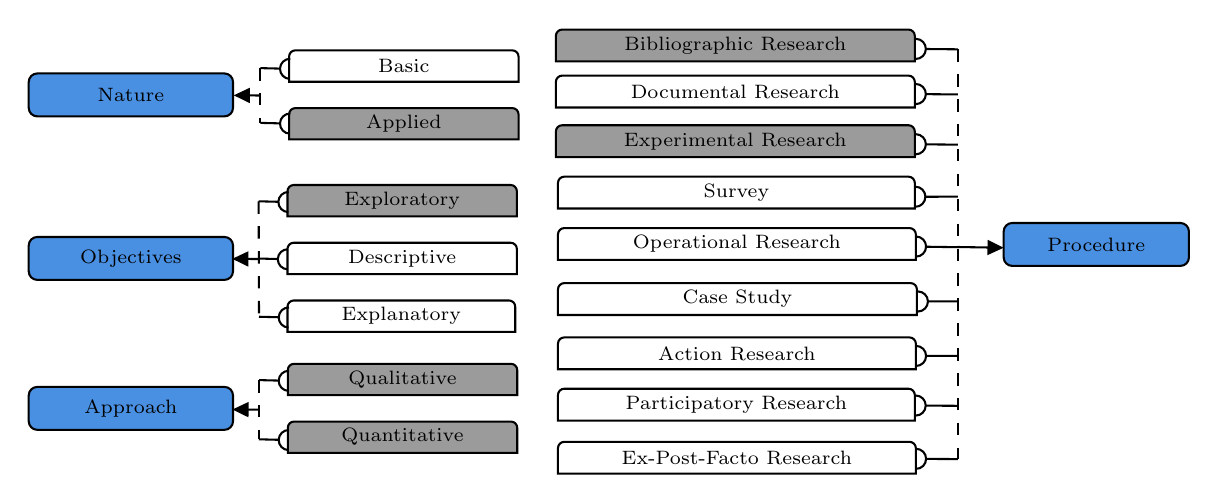
\begin{tikzpicture}[x=0.65pt,y=0.65pt,yscale=-1,xscale=1]
%uncomment if require: \path (0,575); %set diagram left start at 0, and has height of 575

%Rounded Rect [id:dp6868135153852797] 
\draw  [fill={rgb, 255:red, 74; green, 144; blue, 226 }  ,fill opacity=1 ] (7.68,232.87) .. controls (7.68,230.24) and (9.82,228.1) .. (12.46,228.1) -- (116.49,228.1) .. controls (119.13,228.1) and (121.26,230.24) .. (121.26,232.87) -- (121.26,247.19) .. controls (121.26,249.83) and (119.13,251.96) .. (116.49,251.96) -- (12.46,251.96) .. controls (9.82,251.96) and (7.68,249.83) .. (7.68,247.19) -- cycle ;
%Rounded Same Side Corner Rect [id:dp20235263087876798] 
\draw  [fill={rgb, 255:red, 155; green, 155; blue, 155 }  ,fill opacity=1 ] (151.71,218.75) .. controls (151.71,216.83) and (153.27,215.26) .. (155.2,215.26) -- (275.77,215.26) .. controls (277.69,215.26) and (279.26,216.83) .. (279.26,218.75) -- (279.26,232.71) .. controls (279.26,232.71) and (279.26,232.71) .. (279.26,232.71) -- (151.71,232.71) .. controls (151.71,232.71) and (151.71,232.71) .. (151.71,232.71) -- cycle ;
%Rounded Same Side Corner Rect [id:dp22264921749728006] 
\draw  [fill={rgb, 255:red, 155; green, 155; blue, 155 }  ,fill opacity=1 ] (151.71,250.85) .. controls (151.71,248.92) and (153.27,247.36) .. (155.2,247.36) -- (275.77,247.36) .. controls (277.69,247.36) and (279.26,248.92) .. (279.26,250.85) -- (279.26,264.8) .. controls (279.26,264.8) and (279.26,264.8) .. (279.26,264.8) -- (151.71,264.8) .. controls (151.71,264.8) and (151.71,264.8) .. (151.71,264.8) -- cycle ;
%Straight Lines [id:da018056161552026495] 
\draw  [dash pattern={on 4.5pt off 4.5pt}]  (135.7,224.32) -- (135.7,257.23) ;
%Straight Lines [id:da9552157097490397] 
\draw    (135.7,257.23) -- (146.65,257.51) ;
\draw [shift={(146.65,257.51)}, rotate = 1.43] [color={rgb, 255:red, 0; green, 0; blue, 0 }  ][line width=0.75]      (5.59,-5.59) .. controls (2.5,-5.59) and (0,-3.09) .. (0,0) .. controls (0,3.09) and (2.5,5.59) .. (5.59,5.59) ;
%Straight Lines [id:da21069933634089733] 
\draw    (135.7,224.32) -- (146.65,224.59) ;
\draw [shift={(146.65,224.59)}, rotate = 1.43] [color={rgb, 255:red, 0; green, 0; blue, 0 }  ][line width=0.75]      (5.59,-5.59) .. controls (2.5,-5.59) and (0,-3.09) .. (0,0) .. controls (0,3.09) and (2.5,5.59) .. (5.59,5.59) ;
%Straight Lines [id:da8681457188355104] 
\draw    (123.96,240.69) -- (135.7,240.77) ;
\draw [shift={(120.96,240.67)}, rotate = 0.41] [fill={rgb, 255:red, 0; green, 0; blue, 0 }  ][line width=0.08]  [draw opacity=0] (8.93,-4.29) -- (0,0) -- (8.93,4.29) -- cycle    ;
%Rounded Rect [id:dp17274903266410435] 
\draw  [fill={rgb, 255:red, 74; green, 144; blue, 226 }  ,fill opacity=1 ] (7.68,58.61) .. controls (7.68,55.98) and (9.82,53.84) .. (12.46,53.84) -- (116.49,53.84) .. controls (119.13,53.84) and (121.26,55.98) .. (121.26,58.61) -- (121.26,72.93) .. controls (121.26,75.57) and (119.13,77.7) .. (116.49,77.7) -- (12.46,77.7) .. controls (9.82,77.7) and (7.68,75.57) .. (7.68,72.93) -- cycle ;
%Rounded Same Side Corner Rect [id:dp1033670153984676] 
\draw  [fill={rgb, 255:red, 255; green, 255; blue, 255 }  ,fill opacity=1 ] (152.44,44.49) .. controls (152.44,42.56) and (154,41) .. (155.93,41) -- (276.5,41) .. controls (278.42,41) and (279.99,42.56) .. (279.99,44.49) -- (279.99,58.45) .. controls (279.99,58.45) and (279.99,58.45) .. (279.99,58.45) -- (152.44,58.45) .. controls (152.44,58.45) and (152.44,58.45) .. (152.44,58.45) -- cycle ;
%Rounded Same Side Corner Rect [id:dp20109757130923] 
\draw  [fill={rgb, 255:red, 155; green, 155; blue, 155 }  ,fill opacity=1 ] (152.44,76.58) .. controls (152.44,74.66) and (154,73.1) .. (155.93,73.1) -- (276.5,73.1) .. controls (278.42,73.1) and (279.99,74.66) .. (279.99,76.58) -- (279.99,90.54) .. controls (279.99,90.54) and (279.99,90.54) .. (279.99,90.54) -- (152.44,90.54) .. controls (152.44,90.54) and (152.44,90.54) .. (152.44,90.54) -- cycle ;
%Straight Lines [id:da14715624443760533] 
\draw  [dash pattern={on 4.5pt off 4.5pt}]  (136.43,50.88) -- (136.43,81.32) ;
%Straight Lines [id:da04430545750204917] 
\draw    (136.43,50.88) -- (147.38,51.15) ;
\draw [shift={(147.38,51.15)}, rotate = 1.43] [color={rgb, 255:red, 0; green, 0; blue, 0 }  ][line width=0.75]      (5.59,-5.59) .. controls (2.5,-5.59) and (0,-3.09) .. (0,0) .. controls (0,3.09) and (2.5,5.59) .. (5.59,5.59) ;
%Straight Lines [id:da2499030907677271] 
\draw    (136.43,81.32) -- (147.38,81.6) ;
\draw [shift={(147.38,81.6)}, rotate = 1.43] [color={rgb, 255:red, 0; green, 0; blue, 0 }  ][line width=0.75]      (5.59,-5.59) .. controls (2.5,-5.59) and (0,-3.09) .. (0,0) .. controls (0,3.09) and (2.5,5.59) .. (5.59,5.59) ;
%Straight Lines [id:da9005600000477889] 
\draw    (124.69,66.02) -- (136.43,66.1) ;
\draw [shift={(121.69,66)}, rotate = 0.41] [fill={rgb, 255:red, 0; green, 0; blue, 0 }  ][line width=0.08]  [draw opacity=0] (8.93,-4.29) -- (0,0) -- (8.93,4.29) -- cycle    ;
%Rounded Rect [id:dp7698866946845346] 
\draw  [fill={rgb, 255:red, 74; green, 144; blue, 226 }  ,fill opacity=1 ] (7.68,149.52) .. controls (7.68,146.88) and (9.82,144.75) .. (12.46,144.75) -- (116.49,144.75) .. controls (119.13,144.75) and (121.26,146.88) .. (121.26,149.52) -- (121.26,163.84) .. controls (121.26,166.47) and (119.13,168.61) .. (116.49,168.61) -- (12.46,168.61) .. controls (9.82,168.61) and (7.68,166.47) .. (7.68,163.84) -- cycle ;
%Rounded Same Side Corner Rect [id:dp8089622800204079] 
\draw  [fill={rgb, 255:red, 155; green, 155; blue, 155 }  ,fill opacity=1 ] (151.53,119.35) .. controls (151.53,117.43) and (153.09,115.86) .. (155.02,115.86) -- (275.58,115.86) .. controls (277.51,115.86) and (279.07,117.43) .. (279.07,119.35) -- (279.07,133.31) .. controls (279.07,133.31) and (279.07,133.31) .. (279.07,133.31) -- (151.53,133.31) .. controls (151.53,133.31) and (151.53,133.31) .. (151.53,133.31) -- cycle ;
%Rounded Same Side Corner Rect [id:dp7327130032523914] 
\draw  [fill={rgb, 255:red, 255; green, 255; blue, 255 }  ,fill opacity=1 ] (151.53,151.45) .. controls (151.53,149.52) and (153.09,147.96) .. (155.02,147.96) -- (275.58,147.96) .. controls (277.51,147.96) and (279.07,149.52) .. (279.07,151.45) -- (279.07,165.4) .. controls (279.07,165.4) and (279.07,165.4) .. (279.07,165.4) -- (151.53,165.4) .. controls (151.53,165.4) and (151.53,165.4) .. (151.53,165.4) -- cycle ;
%Rounded Same Side Corner Rect [id:dp9942058967704934] 
\draw  [fill={rgb, 255:red, 255; green, 255; blue, 255 }  ,fill opacity=1 ] (151.53,183.54) .. controls (151.53,181.61) and (153.09,180.05) .. (155.02,180.05) -- (274.65,180.05) .. controls (276.58,180.05) and (278.14,181.61) .. (278.14,183.54) -- (278.14,197.49) .. controls (278.14,197.49) and (278.14,197.49) .. (278.14,197.49) -- (151.53,197.49) .. controls (151.53,197.49) and (151.53,197.49) .. (151.53,197.49) -- cycle ;
%Straight Lines [id:da046315945124983715] 
\draw  [dash pattern={on 4.5pt off 4.5pt}]  (135.52,124.92) -- (135.7,189.1) ;
%Straight Lines [id:da3895169007155348] 
\draw    (135.52,124.92) -- (146.47,125.19) ;
\draw [shift={(146.47,125.19)}, rotate = 1.43] [color={rgb, 255:red, 0; green, 0; blue, 0 }  ][line width=0.75]      (5.59,-5.59) .. controls (2.5,-5.59) and (0,-3.09) .. (0,0) .. controls (0,3.09) and (2.5,5.59) .. (5.59,5.59) ;
%Straight Lines [id:da8228559171741872] 
\draw    (135.21,156.73) -- (146.16,157.01) ;
\draw [shift={(146.16,157.01)}, rotate = 1.43] [color={rgb, 255:red, 0; green, 0; blue, 0 }  ][line width=0.75]      (5.59,-5.59) .. controls (2.5,-5.59) and (0,-3.09) .. (0,0) .. controls (0,3.09) and (2.5,5.59) .. (5.59,5.59) ;
%Straight Lines [id:da7567728090403563] 
\draw    (135.7,189.1) -- (146.66,189.38) ;
\draw [shift={(146.66,189.38)}, rotate = 1.43] [color={rgb, 255:red, 0; green, 0; blue, 0 }  ][line width=0.75]      (5.59,-5.59) .. controls (2.5,-5.59) and (0,-3.09) .. (0,0) .. controls (0,3.09) and (2.5,5.59) .. (5.59,5.59) ;
%Straight Lines [id:da9898362078103982] 
\draw    (123.87,156.92) -- (135.61,157.01) ;
\draw [shift={(120.87,156.9)}, rotate = 0.41] [fill={rgb, 255:red, 0; green, 0; blue, 0 }  ][line width=0.08]  [draw opacity=0] (8.93,-4.29) -- (0,0) -- (8.93,4.29) -- cycle    ;
%Rounded Rect [id:dp491721211671053] 
\draw  [fill={rgb, 255:red, 74; green, 144; blue, 226 }  ,fill opacity=1 ] (549.68,141.74) .. controls (549.68,139.11) and (551.81,136.97) .. (554.45,136.97) -- (647.91,136.97) .. controls (650.55,136.97) and (652.68,139.11) .. (652.68,141.74) -- (652.68,156.06) .. controls (652.68,158.7) and (650.55,160.83) .. (647.91,160.83) -- (554.45,160.83) .. controls (551.81,160.83) and (549.68,158.7) .. (549.68,156.06) -- cycle ;
%Rounded Same Side Corner Rect [id:dp35595655488138744] 
\draw  [fill={rgb, 255:red, 155; green, 155; blue, 155 }  ,fill opacity=1 ] (300.73,33) .. controls (300.73,31.04) and (302.31,29.45) .. (304.27,29.45) -- (496.74,29.45) .. controls (498.7,29.45) and (500.29,31.04) .. (500.29,33) -- (500.29,47.17) .. controls (500.29,47.17) and (500.29,47.17) .. (500.29,47.17) -- (300.73,47.17) .. controls (300.73,47.17) and (300.73,47.17) .. (300.73,47.17) -- cycle ;
%Rounded Same Side Corner Rect [id:dp00202486106971711] 
\draw  [fill={rgb, 255:red, 255; green, 255; blue, 255 }  ,fill opacity=1 ] (300.73,58.59) .. controls (300.73,56.63) and (302.31,55.04) .. (304.27,55.04) -- (496.74,55.04) .. controls (498.7,55.04) and (500.29,56.63) .. (500.29,58.59) -- (500.29,72.76) .. controls (500.29,72.76) and (500.29,72.76) .. (500.29,72.76) -- (300.73,72.76) .. controls (300.73,72.76) and (300.73,72.76) .. (300.73,72.76) -- cycle ;
%Rounded Same Side Corner Rect [id:dp4583902576750212] 
\draw  [fill={rgb, 255:red, 155; green, 155; blue, 155 }  ,fill opacity=1 ] (300.73,86.17) .. controls (300.73,84.22) and (302.31,82.63) .. (304.27,82.63) -- (496.74,82.63) .. controls (498.7,82.63) and (500.29,84.22) .. (500.29,86.17) -- (500.29,100.34) .. controls (500.29,100.34) and (500.29,100.34) .. (500.29,100.34) -- (300.73,100.34) .. controls (300.73,100.34) and (300.73,100.34) .. (300.73,100.34) -- cycle ;
%Rounded Same Side Corner Rect [id:dp07252697986537204] 
\draw  [fill={rgb, 255:red, 255; green, 255; blue, 255 }  ,fill opacity=1 ] (301.9,114.76) .. controls (301.9,112.8) and (303.48,111.22) .. (305.44,111.22) -- (496.74,111.22) .. controls (498.7,111.22) and (500.29,112.8) .. (500.29,114.76) -- (500.29,128.93) .. controls (500.29,128.93) and (500.29,128.93) .. (500.29,128.93) -- (301.9,128.93) .. controls (301.9,128.93) and (301.9,128.93) .. (301.9,128.93) -- cycle ;
%Rounded Same Side Corner Rect [id:dp3622010030980434] 
\draw  [fill={rgb, 255:red, 255; green, 255; blue, 255 }  ,fill opacity=1 ] (301.9,143.35) .. controls (301.9,141.39) and (303.48,139.81) .. (305.44,139.81) -- (497.33,139.81) .. controls (499.29,139.81) and (500.87,141.39) .. (500.87,143.35) -- (500.87,157.52) .. controls (500.87,157.52) and (500.87,157.52) .. (500.87,157.52) -- (301.9,157.52) .. controls (301.9,157.52) and (301.9,157.52) .. (301.9,157.52) -- cycle ;
%Rounded Same Side Corner Rect [id:dp79526073007951] 
\draw  [fill={rgb, 255:red, 255; green, 255; blue, 255 }  ,fill opacity=1 ] (301.9,173.94) .. controls (301.9,171.98) and (303.48,170.39) .. (305.44,170.39) -- (497.92,170.39) .. controls (499.87,170.39) and (501.46,171.98) .. (501.46,173.94) -- (501.46,188.11) .. controls (501.46,188.11) and (501.46,188.11) .. (501.46,188.11) -- (301.9,188.11) .. controls (301.9,188.11) and (301.9,188.11) .. (301.9,188.11) -- cycle ;
%Rounded Same Side Corner Rect [id:dp4163024414983818] 
\draw  [fill={rgb, 255:red, 255; green, 255; blue, 255 }  ,fill opacity=1 ] (301.9,204.13) .. controls (301.9,202.17) and (303.48,200.59) .. (305.44,200.59) -- (497.33,200.59) .. controls (499.29,200.59) and (500.87,202.17) .. (500.87,204.13) -- (500.87,218.3) .. controls (500.87,218.3) and (500.87,218.3) .. (500.87,218.3) -- (301.9,218.3) .. controls (301.9,218.3) and (301.9,218.3) .. (301.9,218.3) -- cycle ;
%Rounded Same Side Corner Rect [id:dp9905230238041782] 
\draw  [fill={rgb, 255:red, 255; green, 255; blue, 255 }  ,fill opacity=1 ] (301.9,232.65) .. controls (301.9,230.7) and (303.48,229.11) .. (305.44,229.11) -- (496.74,229.11) .. controls (498.7,229.11) and (500.29,230.7) .. (500.29,232.65) -- (500.29,246.83) .. controls (500.29,246.83) and (500.29,246.83) .. (500.29,246.83) -- (301.9,246.83) .. controls (301.9,246.83) and (301.9,246.83) .. (301.9,246.83) -- cycle ;
%Rounded Same Side Corner Rect [id:dp10898668174723891] 
\draw  [fill={rgb, 255:red, 255; green, 255; blue, 255 }  ,fill opacity=1 ] (301.9,262.18) .. controls (301.9,260.22) and (303.48,258.64) .. (305.44,258.64) -- (497.33,258.64) .. controls (499.29,258.64) and (500.87,260.22) .. (500.87,262.18) -- (500.87,276.35) .. controls (500.87,276.35) and (500.87,276.35) .. (500.87,276.35) -- (301.9,276.35) .. controls (301.9,276.35) and (301.9,276.35) .. (301.9,276.35) -- cycle ;
%Straight Lines [id:da3798370991300257] 
\draw    (524.28,268.23) -- (506.55,268.12) ;
\draw [shift={(506.55,268.12)}, rotate = 180.35] [color={rgb, 255:red, 0; green, 0; blue, 0 }  ][line width=0.75]      (5.59,-5.59) .. controls (2.5,-5.59) and (0,-3.09) .. (0,0) .. controls (0,3.09) and (2.5,5.59) .. (5.59,5.59) ;
%Straight Lines [id:da7243916707412472] 
\draw  [dash pattern={on 4.5pt off 4.5pt}]  (524.28,40.43) -- (524.28,268.23) ;
%Straight Lines [id:da6462001191130786] 
\draw    (524.28,238.61) -- (506.35,238.5) ;
\draw [shift={(506.35,238.5)}, rotate = 180.35] [color={rgb, 255:red, 0; green, 0; blue, 0 }  ][line width=0.75]      (5.59,-5.59) .. controls (2.5,-5.59) and (0,-3.09) .. (0,0) .. controls (0,3.09) and (2.5,5.59) .. (5.59,5.59) ;
%Straight Lines [id:da3380864013747653] 
\draw    (524.28,210.81) -- (506.55,210.86) ;
\draw [shift={(506.55,210.86)}, rotate = 179.82] [color={rgb, 255:red, 0; green, 0; blue, 0 }  ][line width=0.75]      (5.59,-5.59) .. controls (2.5,-5.59) and (0,-3.09) .. (0,0) .. controls (0,3.09) and (2.5,5.59) .. (5.59,5.59) ;
%Straight Lines [id:da885883100870726] 
\draw    (524.28,180.54) -- (507.57,180.59) ;
\draw [shift={(507.57,180.59)}, rotate = 179.81] [color={rgb, 255:red, 0; green, 0; blue, 0 }  ][line width=0.75]      (5.59,-5.59) .. controls (2.5,-5.59) and (0,-3.09) .. (0,0) .. controls (0,3.09) and (2.5,5.59) .. (5.59,5.59) ;
%Straight Lines [id:da6876534243633374] 
\draw    (524.28,150.44) -- (506.55,150.17) ;
\draw [shift={(506.55,150.17)}, rotate = 180.89] [color={rgb, 255:red, 0; green, 0; blue, 0 }  ][line width=0.75]      (5.59,-5.59) .. controls (2.5,-5.59) and (0,-3.09) .. (0,0) .. controls (0,3.09) and (2.5,5.59) .. (5.59,5.59) ;
%Straight Lines [id:da4341764738295175] 
\draw    (524.28,122.35) -- (506.17,122.38) ;
\draw [shift={(506.17,122.38)}, rotate = 179.89] [color={rgb, 255:red, 0; green, 0; blue, 0 }  ][line width=0.75]      (5.59,-5.59) .. controls (2.5,-5.59) and (0,-3.09) .. (0,0) .. controls (0,3.09) and (2.5,5.59) .. (5.59,5.59) ;
%Straight Lines [id:da17881011353561926] 
\draw    (524.28,93.43) -- (506.43,93.26) ;
\draw [shift={(506.43,93.26)}, rotate = 180.55] [color={rgb, 255:red, 0; green, 0; blue, 0 }  ][line width=0.75]      (5.59,-5.59) .. controls (2.5,-5.59) and (0,-3.09) .. (0,0) .. controls (0,3.09) and (2.5,5.59) .. (5.59,5.59) ;
%Straight Lines [id:da9022272397272932] 
\draw    (524.28,65.52) -- (506.43,65.35) ;
\draw [shift={(506.43,65.35)}, rotate = 180.55] [color={rgb, 255:red, 0; green, 0; blue, 0 }  ][line width=0.75]      (5.59,-5.59) .. controls (2.5,-5.59) and (0,-3.09) .. (0,0) .. controls (0,3.09) and (2.5,5.59) .. (5.59,5.59) ;
%Straight Lines [id:da1804325455133604] 
\draw    (524.28,40.43) -- (506.43,40.25) ;
\draw [shift={(506.43,40.25)}, rotate = 180.55] [color={rgb, 255:red, 0; green, 0; blue, 0 }  ][line width=0.75]      (5.59,-5.59) .. controls (2.5,-5.59) and (0,-3.09) .. (0,0) .. controls (0,3.09) and (2.5,5.59) .. (5.59,5.59) ;
%Straight Lines [id:da5547588201230154] 
\draw    (524.28,150.33) -- (546.62,150.69) ;
\draw [shift={(549.62,150.74)}, rotate = 180.93] [fill={rgb, 255:red, 0; green, 0; blue, 0 }  ][line width=0.08]  [draw opacity=0] (8.93,-4.29) -- (0,0) -- (8.93,4.29) -- cycle    ;

% Text Node
\draw (216.21,49.73) node  [font=\scriptsize] [align=left] {Basic};
% Text Node
\draw (216.21,81.82) node  [font=\scriptsize] [align=left] {Applied};
% Text Node
\draw (215.3,124.59) node  [font=\scriptsize] [align=left] {Exploratory};
% Text Node
\draw (215.3,156.68) node  [font=\scriptsize] [align=left] {Descriptive};
% Text Node
\draw (214.84,188.77) node  [font=\scriptsize] [align=left] {Explanatory};
% Text Node
\draw (215.48,223.99) node  [font=\scriptsize] [align=left] {Qualitative};
% Text Node
\draw (215.48,256.08) node  [font=\scriptsize] [align=left] {Quantitative};
% Text Node
\draw (64.47,65.77) node  [font=\scriptsize] [align=left] {Nature};
% Text Node
\draw (64.47,156.68) node  [font=\scriptsize] [align=left] {Objectives};
% Text Node
\draw (64.47,240.03) node  [font=\scriptsize] [align=left] {Approach};
% Text Node
\draw (400.51,38.31) node  [font=\scriptsize] [align=left] {Bibliographic Research};
% Text Node
\draw (400.51,63.9) node  [font=\scriptsize] [align=left] {Documental Research};
% Text Node
\draw (400.51,91.49) node  [font=\scriptsize] [align=left] {Experimental Research};
% Text Node
\draw (401.09,120.07) node  [font=\scriptsize] [align=left] {Survey};
% Text Node
\draw (401.38,148.66) node  [font=\scriptsize] [align=left] {Operational Research};
% Text Node
\draw (401.68,179.25) node  [font=\scriptsize] [align=left] {Case Study};
% Text Node
\draw (401.38,209.45) node  [font=\scriptsize] [align=left] {Action Research};
% Text Node
\draw (401.09,237.97) node  [font=\scriptsize] [align=left] {Participatory Research};
% Text Node
\draw (401.38,267.49) node  [font=\scriptsize] [align=left] {Ex-Post-Facto Research};
% Text Node
\draw (601.18,148.9) node  [font=\scriptsize] [align=left] {Procedure};


\end{tikzpicture}

    \fonte{Adapted from \cite{Prodanov:2013}.}
    \label{fig:ResearchClassification}
\end{figure}

% Segundo \citeonline{Prodanov:2013}, nenhum tipo de pesquisa é autossuficiente, sendo então necessário a mescla de diferentes tipos, tendo um ou outro ponto mais acentuado, para a obtenção de resultados satisfatórios. 
% Os métodos escolhidos determinam os procedimentos que devem ser utilizados, tanto na coleta de dados e informações quanto na análise.
%According to \cite{Prodanov:2013}, no type of research is self-sufficient, so it is necessary to mix different types, with one or another more accentuated points to obtain satisfactory results.
According to \cite{Prodanov:2013}, no type of research is self-sufficient, so it is necessary to mix different types with more accentuated points to obtain satisfactory results.
The chosen methods determine the procedures that should be used, both in analysis and in data and information collection.

% No que se refere a sua natureza, uma pesquisa pode ser básica ou aplicada. 
% Este trabalho propõe uma ferramenta que utiliza uma DSL, gerando uma ferramenta prática para solucionar algo específico e, sendo assim, pode ser categorizada como uma pesquisa de natureza aplicada.
In terms of its nature, research can be basic or applied.
%This study proposes a tool that uses a DSL, generating a practical tool to solve something specific and, therefore, it can be categorized as an applied research.
This study proposes a tool that uses a DSL, generating a practical tool to solve something specific and, therefore, we can categorize it as applied research.

% Do ponto de vista dos seus objetivos, uma pesquisa pode ser classificada como exploratória, descritiva ou explicativa. 
% Este estudo tem como finalidade oferecer mais informações sobre o assunto que investiga, logo, é uma pesquisa exploratória. 
From the point of view of its objectives, research classifies as exploratory, descriptive, or explanatory. This study aims to provide more information on the subject it investigates. Hence, it is explanatory research.

% A abordagem do problema pode classificar a pesquisa em quantitativa ou qualitativa. 
% Este trabalho aplica os conceitos de ambas as categorias.
% Isso ocorre a partir das avaliações, tanto preliminar quanto a experimental planejada para o futuro, onde é necessário fazer observações empíricas para interpretar a avaliação de uso dos sujeitos participantes, e métodos estatísticos para avaliar os modelos produzidos.
The problem approach can classify the research into quantitative or qualitative.
This study applies the concepts of both categories.
It occurs from experimental evaluations, both preliminary and planned for the future, where it is necessary to make empirical assessment observations to interpret the participant experiences and also statistical methods to evaluate the models produced.

% Por fim, com relação a seu procedimentos técnicos, uma pesquisa pode ser categorizada como pesquisa bibliográfica, documental, experimental, do tipo levantamento, também chamada de survey, pesquisa operacional, estudo de caso, pesquisa ex-post-facto, pesquisa-ação e pesquisa participante. 
% Este trabalho realiza uma pesquisa bibliográfica nas atividades executadas para o levantamento de sua base teórica e, além disso, executa uma pesquisa experimental na etapa de avaliação da ferramenta final produzida.
% Finally, with regard to its technical procedures, a research can be categorized as bibliographical, documentary, experimental, survey-type research, also called survey, operational research, case study, ex-post-facto research, action research and participant research.
% This work performs a bibliographical research on the activities performed to survey its theoretical basis and, in addition, performs an experimental research in the evaluation stage of the final tool produced.
Finally, technical procedures group research categories as bibliographical, documentary, experimental, survey-type research, also called survey, operational research, case study, \textit{ex-post-facto} research, action research and participant research.
Hence, this study performs a bibliographical research, \textit{i.e.} the activities performed to survey its theoretical framework. 
Besides, we carry out an experimental research in the evaluation stage of the tool proposed.

%------------------------------------------------------------------------------
\section{Research Design}\label{met:researchdesign}
%------------------------------------------------------------------------------

% Na Figura \ref{fig:ResearchDesign} é apresentado o nosso projeto de pesquisa. 
% Dividimos este projeto em quatro (4) grupos de atividades. 
In Figure \ref{fig:ResearchDesign} our research design is presented.
We have divided this project into four (4) groups of activities.

% O primeiro grupo corresponde a fase de concepção.
% Esta fase compreende na identificação do problema e motivação, no estabelecimento dos objetivos e a definição da estrutura do estudo.
% Para a criação de uma base teórica foram realizadas três atividades em paralelo, sendo o estudo sobre modelagem de projeto de bancos de dados, da engenharia dirigida por modelos e a execução de um mapeamento sistemático de literatura buscando mecanismos de transformação de modelos de bancos de dados relacionais.
The first group corresponds to the design phase.
This phase covers the identification of the problem and motivation, the establishment of objectives and the definition of the study structure.
To create a theoretical framework, three activities were carried out in parallel, namely the study of \ac{db} design modeling, model-driven engineering and the execution of a systematic literature mapping seeking mechanisms for transforming relational \ac{db} models.

% O segundo grupo corresponde a etapa de projeto e desenvolvimento da ferramenta.
% Foram identificados os requisitos, definida a arquitetura para então dar-se início no desenvolvimento da ferramenta. 
% De forma paralela, um protótipo passou por uma avaliação preliminar, descrita no Capítulo \ref{chap:evaluation}.
% Após ter os resultados analisados, provenientes da avaliação preliminar, é então gerado uma versão estável da ferramenta.
The second group covers the design and development stage of the tool.
The requirements were identified, the architecture was defined and then the development of the tool started.
In parallel, a prototype underwent a preliminary evaluation, described in Chapter \ref{chap:experiments}.
After having analyzed the results from the preliminary evaluation, a stable version of the tool is then generated.

% No terceiro grupo estão as atividades correspondentes a um experimento controlado ao qual esta versão estável será submetida, com o objetivo de avaliar todas as funções desenvolvidas. 
% Isso corresponde também a avaliação dos artefatos produzidos pelos geradores implementados: 
% È importante ressaltar que nenhum destes artefatos foram considerados na avaliação preliminar.
% In the third group are the activities corresponding to a controlled experiment to which this stable version will be submitted, with the objective of assess all the developed functions.
% This also corresponds to the evaluation of the artifacts produced by the implemented generators that were not considered in the preliminary evaluation:
In the third group are the activities corresponding to a controlled experiment, in which we will submit this stable version, intending to evaluate all its features developed.
It is also noteworthy that this corresponds to the evaluation of artifacts produced by the implemented generators, which we not considered in the preliminary evaluation:

% \begin{itemize}
%     \item diagramas do modelo conceitual;
%     \item modelos lógicos em texto, no formato html;
%     \item modelos DDL (SQL) para DBMS específicos;
% \end{itemize}

\begin{itemize}
     \item Conceptual model diagrams;
     \item Logical textual models in \ac{html} format;
     \item DDL (\ac{sql}) templates for specific \acp{dbms}.
\end{itemize}

\begin{figure}[!htb]
    \centering
    \caption{Research design.}
    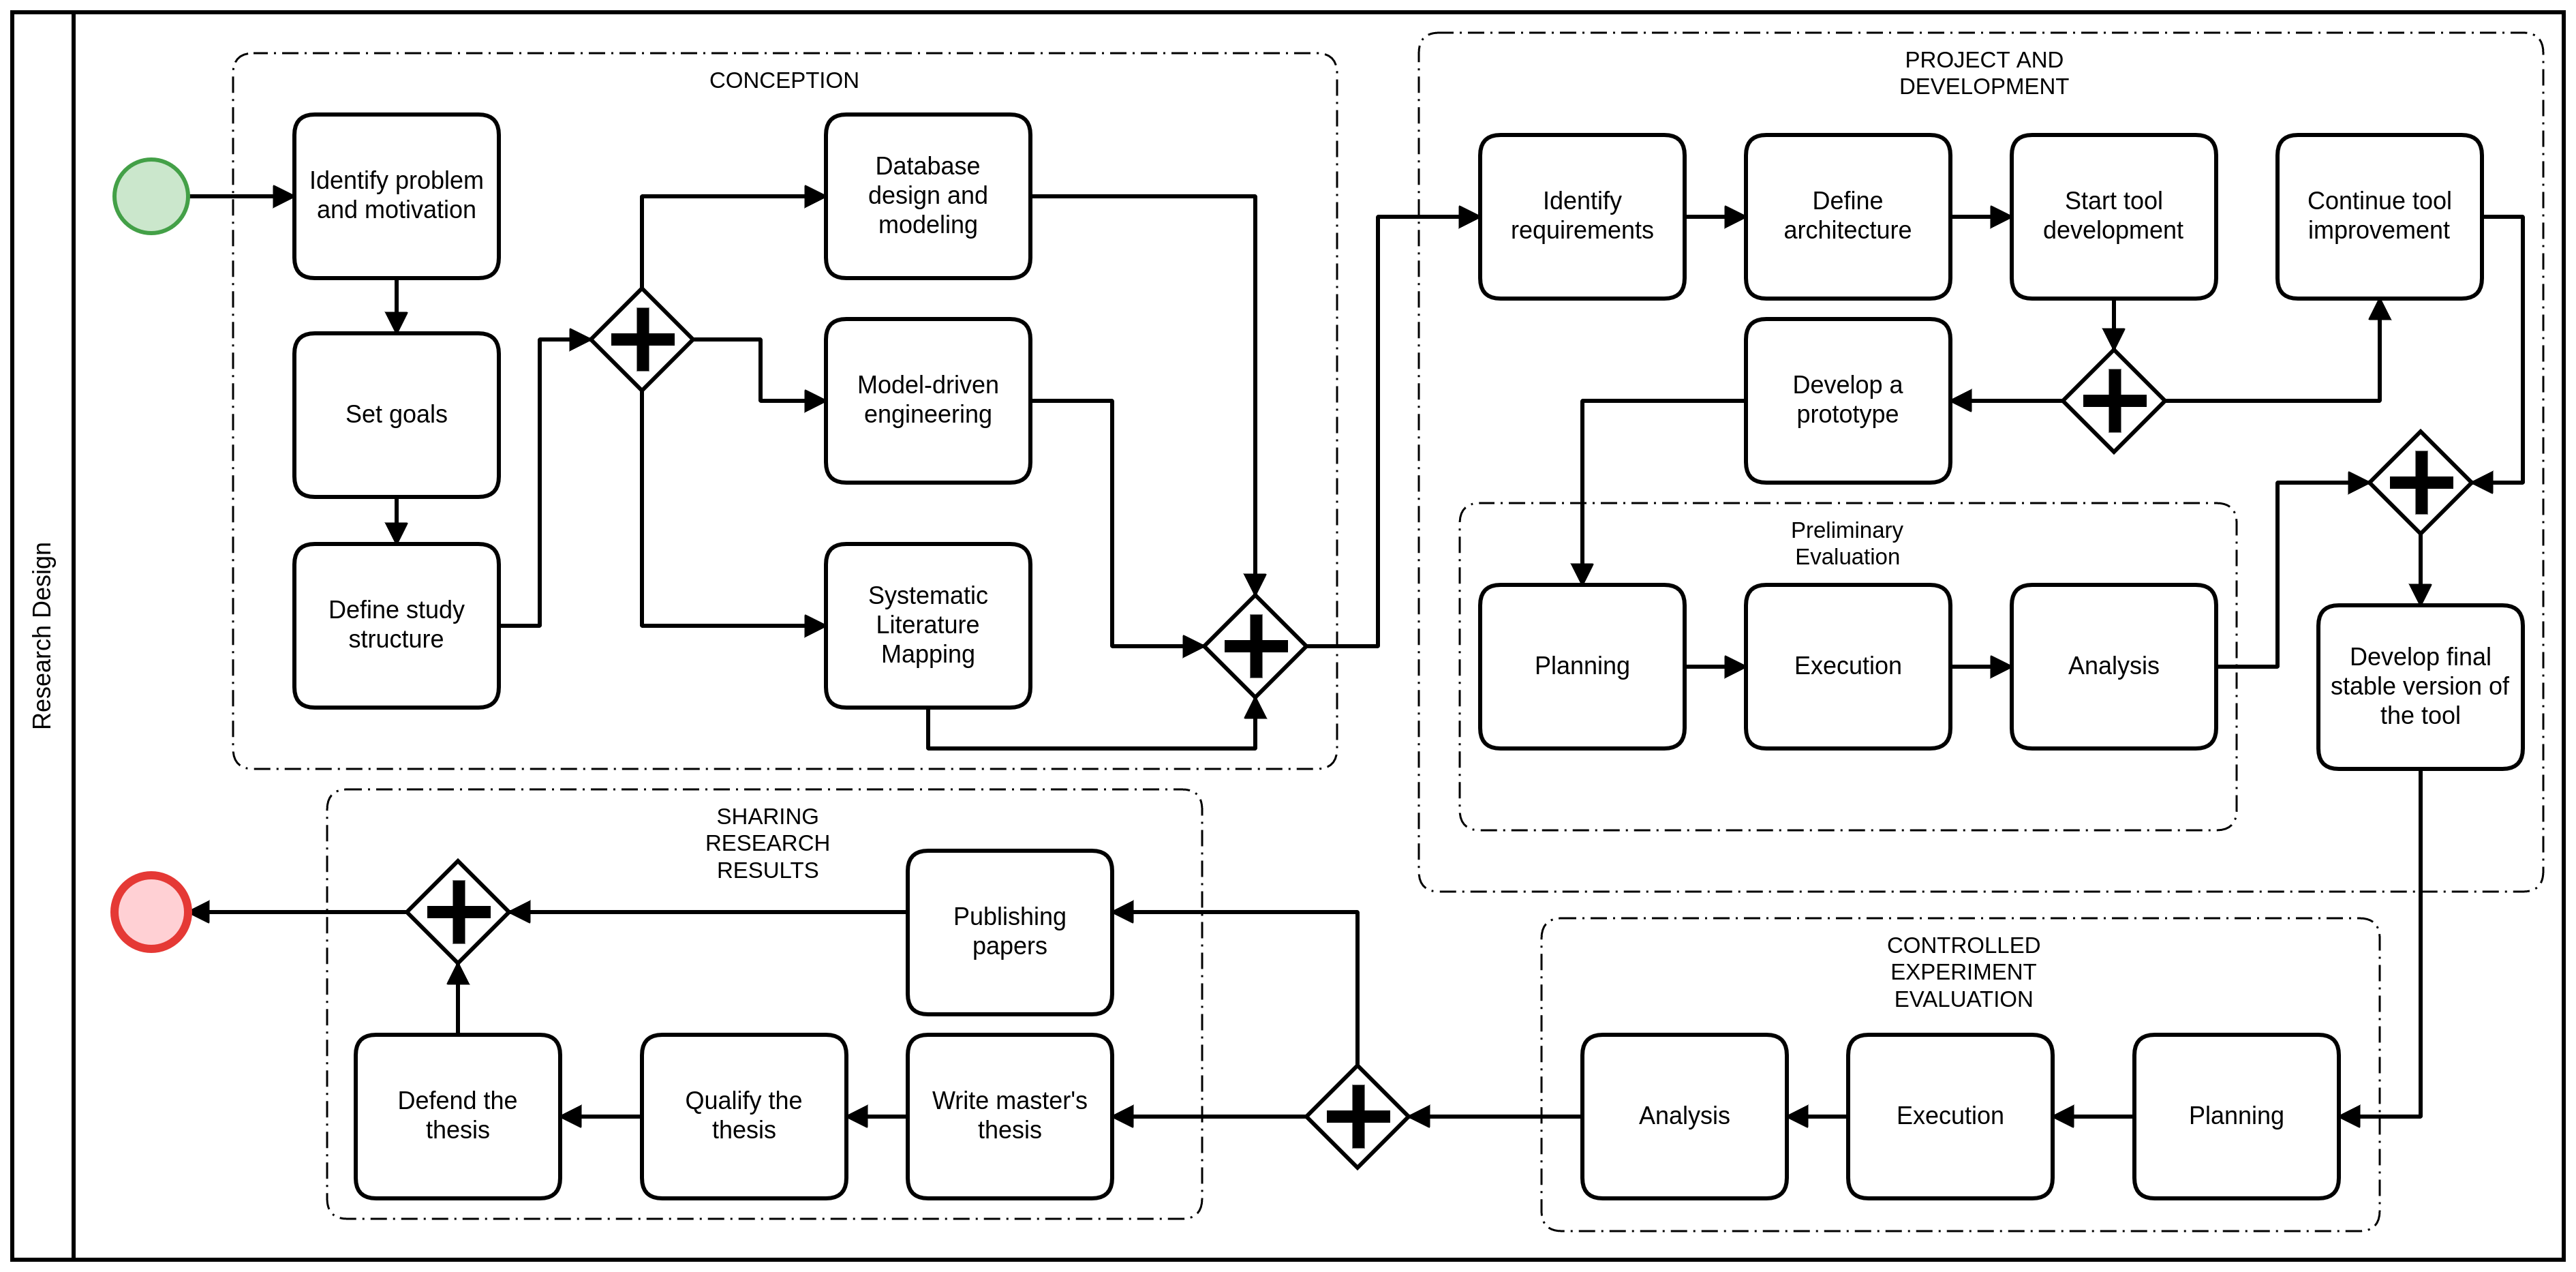
\includegraphics[width=1\textwidth]{img/ResearchDesign.png}
    \fonte{Author.}
    \label{fig:ResearchDesign}
\end{figure}

% Finalmente, o quarto grupo corresponde a divulgação dos resultados da pesquisa desenvolvida.
% Entre as atividades estão a escrita da dissertação e publicação de artigos em eventos científicos.
Finally, the fourth group corresponds to the dissemination of the results of the developed research.
Among the activities, we highlight the writing of the master's thesis and the paper's publishing in scientific events.

%------------------------------------------------------------------------------
\section{Schedule}\label{met:schedule}
% 2021/02 previsto disciplina de BD em CC e ES
% O orientador é o professor da disciplina
% talvez chamar avaliação experimental
%------------------------------------------------------------------------------

% A Tabela \ref{tab:tableSchedule} apresenta o cronograma elaborado para as principais atividades previstas para a realização da dissertação de mestrado.
% As atividades são detalhadas quanto a sua duração conforme os meses que necessitam para serem completadas.
% Table \ref{tab:schedule} presents the schedule elaborated for the main activities foreseen for the accomplishment of the master's thesis.
% Activities are detailed in terms of duration according to the months they need to be completed.
Table \ref{tab:schedule} presents the schedule elaborated for the main activities foreseen to accomplish the master's thesis.
We detailed the activities in terms of duration according to the months they need to be completed.

\section{Chapter Summary}\label{met:lessons}
% Descrever aprendizados
% se for descrever o capitulo, Chapter Summary

% Neste capítulo, apresentamos nossa metodologia de pesquisa.
% A classificação da pesquisa é importante para a realização adequada do planejamento das atividades necessárias para atingir o objetivo proposto neste estudo.
% Sendo assim, a partir de uma visão de alto nível de toda a nossa pesquisa é possível que um cronograma temporal seja detalhado, explicitando cada tarefa que deve ocorrer.
% In this chapter, we present our research methodology.
% The research classification is important for the proper planning of activities necessary to achieve the objective proposed in this study.
% Thus, from a high-level view of all our research, it is possible that a time schedule is detailed, explaining each task that must take place.
In this chapter, we present our research methodology.
The research classification is relevant to properly plan activities necessary to achieve the objective proposed in this study.
Thus, from a high-level view of our entire research, we detail a schedule, explaining each task that must take place.

\begin{landscape}
\begin{table}[!htb]
	\centering
	\caption[Schedule.]{Schedule.}
	\label{tab:schedule}
	\resizebox{1.5\textwidth}{!}{\begin{tabular}{lc|cccccc|cccccc|cccccc|cc}
		\bottomrule
		\rowcolor[HTML]{C0C0C0}
		 & \multicolumn{1}{c|}{\textbf{2020/1}} & \multicolumn{6}{c|}{\textbf{2020/2}} & \multicolumn{6}{c|}{\textbf{2021/1}} & \multicolumn{6}{c|}{\textbf{2021/2}} & \multicolumn{2}{c}{\textbf{2022/1}}\\
		%\rowcolor[HTML]{C0C0C0}
		\textbf{Tasks} & \textbf{Jun} & \textbf{Jul} & \textbf{Aug} & \textbf{Sep} & \textbf{Oct} & \textbf{Nov} & \textbf{Dec} & \textbf{Jan} & \textbf{Feb} & \textbf{Mar} &  \textbf{Apr} & \textbf{May} & \textbf{Jun} & \textbf{Jul} & \textbf{Aug} & \textbf{Sep} & \textbf{Oct} & \textbf{Nov} & \textbf{Dec} & \textbf{Jan} & \textbf{Feb} \\ \hline
		
		\rowcolor[HTML]{C0C0C0}
		Tool Development & \checkmark & \checkmark & \checkmark & \checkmark & \checkmark & \checkmark & \checkmark & \checkmark & \checkmark & \checkmark & \checkmark & \checkmark & \checkmark & \checkmark & \checkmark & \checkmark & \checkmark & \checkmark & - & - & - \\
		
		Systematic Literature Mapping & - & - & - & \checkmark & \checkmark & \checkmark & \checkmark & - & - & - & - & - & - & - & - & - & - & - & - & - & - \\
		
		\rowcolor[HTML]{C0C0C0}
		Controlled Experiment 1 Planning & - & - & - & - & - & - & - & \checkmark & \checkmark & - & - & - & - & - & - & - & - & - & - & - & - \\
		
		Controlled Experiment 1 Execution & - & - & - & - & - & - & - & - & \checkmark & - & - & - & - & - & - & - & - & - & - & - & - \\
		
		\rowcolor[HTML]{C0C0C0}
		Controlled Experiment 1 Analysis & - & - & - & - & - & - & - & - & \checkmark & \checkmark & - & - & - & - & - & - & - & - & - & - & - \\
		
		Controlled Experiment 2 Planning & - & - & - & - & - & - & - & - & - & - & - & - & - & - & - & - & \checkmark & \checkmark & - & - & - \\
		
		\rowcolor[HTML]{C0C0C0}
		Controlled Experiment 2 Execution & - & - & - & - & - & - & - & - & - & - & - & - & - & - & - & - & - & \checkmark & \checkmark & - & - \\

		Controlled Experiment 2 Analysis & - & - & - & - & - & - & - & - & - & - & - & - & - & - & - & - & - & - & \checkmark & \checkmark & - \\
		
		\rowcolor[HTML]{C0C0C0}
		Writing and Publishing Articles & - & - & \checkmark & \checkmark & \checkmark & \checkmark & \checkmark & \checkmark & \checkmark & \checkmark & \checkmark & \checkmark & \checkmark & \checkmark & \checkmark & \checkmark & - & - & - & - & - \\
		
		Write Master's Thesis & - & - & - & - & - & - & - & - & - & - & - & - & - & - & - & - & - & \checkmark & \checkmark & \checkmark & \checkmark \\
		
		\toprule
	\end{tabular}}
\end{table}
\fonte{Author}
\end{landscape}